
\section{Introduction}
\label{physics}

The hadronization process by which parton fragment into hadrons is 
experimentally well studied and fragmentation functions fitted from 
data are measured on a large kinematic range~\cite{Albino:2008fy}.
Nevertheless, the hadron formation is a non perturbative process and can not 
be theoritically described, only a global picture 
(see figure \ref{fig:hadro}) can be drawn for
energies above the resonance region. In deep inelastic scattering the
virtual photon interact with a quark which propagate quasi-free emitting
gluons during the 
so-called production time. After neutralizing its color the quark become 
a pre-hadron which will eventualy form a hadron after the formation time.
On nuclear target the process of hadronization occurs, at least partly, in 
nuclear matter, then one can extract the production time using the different 
behaviour of quarks and colorless pre-hadrons in medium. The measurement of
pions is especially suited to lead that kind of analysis because they are easy
to detect and abundant in deep inelastic scattering.

\begin{figure}[htbp]
\centering
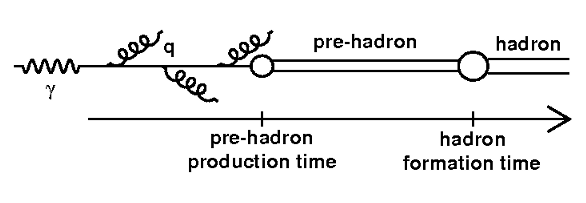
\includegraphics[width=10cm] {fig/hadro.png} 
\caption {Sketch of the hadronization process.}
\label{fig:hadro}
\end{figure}

The hadronization in nuclear matter is a key process in QCD also
because it leads to a major theoritical uncertainty in numerous measurements.
In heavy ion collisions, the measured hadrons are produced in hot and evolving 
medium, the models describing those collisions can be tested in deep inelatic scattering 
where the size of the medium is stable and known. Quantitative
understanding of the hadronization in nuclei is also of interest for
neutrino experiment which often use nuclei to maximize their cross section.
The hadronization can give important information about the 
nuclei through quark energy loss, for exemple \cite{Arleo:2003yf} link 
energy loss with gluon density and \cite{Kopeliovich:2010aa} link the $\Delta \langle
P_T^2 \rangle$ with the saturation scale. Other models \cite{Gallmeister:2007an}
can give information about how the pre-hadron evolve into hadron but are based
on very different assomptions, therefore it is very important to discriminate between
models. 

In order to constrain the existing models we extract our results
using tight multi-dimensional binning. 
The importance of the EG2 data comes from its high statistics which permit, 
this multi-dimensional measurement of both pions on a 
large kinematic range.

We present in section \ref{sec:theo} the different familly of models describing
hadronization in nuclear matter then in section \ref{sec:exp} we make a rapid
overview of the published data on the topic. For more detailed information we 
refer the reader to the review from Accardi {\it et al.} \cite{Accardi:2009qv}.


\subsection{Kinetic Variables and Observables}

In this analysis we use the following semi-inclusive DIS variables:
\begin{itemize}
 \item $\nu = E_i - E_f$ with $E_i$ the beam energy and $E_f$ the scattered electron energy,
 \item $Q^2 = 4 E_i E_f \sin ^2(\theta_e / 2)$ with $\theta_e$ the scattered electron angle with the beam line,
 \item $x_{Bj} = {{Q^2} \over {2 M_n \nu}}$ with $M_n$ the nucleon mass,
 \item $W^2 = M_n^2 - Q^2 + 2 M_n \nu$
 \item $z_h = E_h / \nu$
 \item $P_T^2$ which is transverse momentum according to the virtual photon
 \item $\phi_h$ the angle between the electronic plan (contain initial and scattered electrons) and the hadronic plan (contain virtual photon and hadron)
 \item $x_F = P_L/P_L^{max}$ the fraction of longitudinal momentum carried by the hadron calculated in respect to the virtual photon direction in the laboratory frame.
\end{itemize}
%TODO Add t

We define the multiplicity ratio as:
\begin{equation}
R_A^h (Q^2,\nu,z_h,P_T^2) = {{N_A^h (Q^2,\nu,z_h,P_T^2) / N_A^e (Q^2,\nu)} 
                       \over {N_D^h (Q^2,\nu,z_h,P_T^2) / N_D^e (Q^2,\nu)}}
\end{equation}
with $N^e_A$ the number of electron measured from a target $A$ and $N_A^h$ the number
of semi-inclusive hadrons $h$ (detection of both an electron and a hadron) from the
target~$A$. The multiplicity ratio represents the attenuation of the hadron $h$ in a 
nuclear target~$A$.
\newline

We define the transverse momentum broadening as:
\begin{equation}
\Delta \langle P_T^2 \rangle = \langle P_T^2 \rangle_A - \langle P_T^2 \rangle_D
\end{equation}
with $\langle P_T^2 \rangle_A$ the mean transverse momentum measured in a target $A$.


\subsection{Theoretical Efforts}
\label{sec:theo}

The different models explaining the data can be separated in three families,
some assume that the quark loose energy in the medium and that either, hadronization occurs
outside the medium or the hadronic interaction is 
negligible, others consider the quark energy loss negligible and consider
only the hadron and pre-hadron absorption and finally some models consider both
interactions. We will give an example of each case to illustrate, for more
detailed information we refer again to \cite{Accardi:2009qv} which is more exaustive and
mention few other models used for RHIC experiments.

In \cite{Wang:2002ri}, E.~Wang and X.-N.~Wang, describe HERMES data using only energy 
loss from the parton, the suppression observed is then due to the fact that a 
lower energy quark will fragment into a lower number of hadrons and a lower 
$z$. That kind of model is used in both RHIC and nDIS and permit a commom 
interpretation of hadron suppression in nuclear matter. Lot of different
calculations of the energy loss exist, the main parameter for those is $\hat q$
(GeV$^2$ fm$^{-1}$) which is the transverse momentum per unit of length of a 
quark after propagating
in nuclear matter, this value is related to the $P_T$ 
broadening observables. The main difficulty for the quark energy loss
models is to have coherent description of both multiplicity ratios and $P_T$ 
broadening. Recent models find a $\hat q$ to reproduce multiplicity ratio
which is bigger than the one necessary to describe transverse momentum broadening.
% TODO Add a ref

The GiBUU model \cite{Gallmeister:2007an} is a transport model based on Boltzmann equation
using hadronic and pre-hadronic interaction in the nuclear matter, with no
quark energy loss involved. This model reproduce very well most of the hadrons, 
however the $\Delta \langle P_T^2 \rangle$ variable is not described at all by 
this hadron absorption models.

B.Z.~Kopeliovich \cite{Kopeliovich:2008uy} describe the process neglegting neither quark 
energy loss or hadron absorption, using transverse momentum and
multiplicity ratios to differenciate the effects. In that case the transverse 
momentum broadening is linked to quark energy loss and the multiplicity ratio
suppression is explained by hadron absorption in medium.

To conclude it is important to point out that no consensus is reached on which 
mecanisms are dominant. It is therefore important to perform precise measurements with
the right observables to solve this problem.


\subsection{Previous Mesurements}
\label{sec:exp}

Hadron multiplicity ratios in nuclei were measured in numerous lepton 
facilities: L.S.~Osborne {\it et al.} \cite{Osborne:1978ai} at SLAC,
L.~Hand {\it et al.} \cite{Hand:1978tx} and the E665 collaboration \cite{Adams:1994ri} at FNAL
and the European Muon Collaboration \cite{Arvidson:1984fz,Ashman:1991cx} at CERN. Those 
measurements revealed the general features of hadronization
in nuclei: we observe a sizeable suppression when
looking at hadron production in nuclei, this suppression is lower at higher
$\nu$ and lower $z$, it can even inverse and be an increased yield at very low $z$. 

The figures \ref{fig:her1}, \ref{fig:her2} and \ref{fig:her3} shows a sample of 
the most recent data from HERMES collaboration \cite{Airapetian:2007vu}, numerous 
hadrons are studied individually and new variables linked with transverse 
momentum are used on top of the usual multiplicity ratio.

\begin{figure}[htbp]
\centering
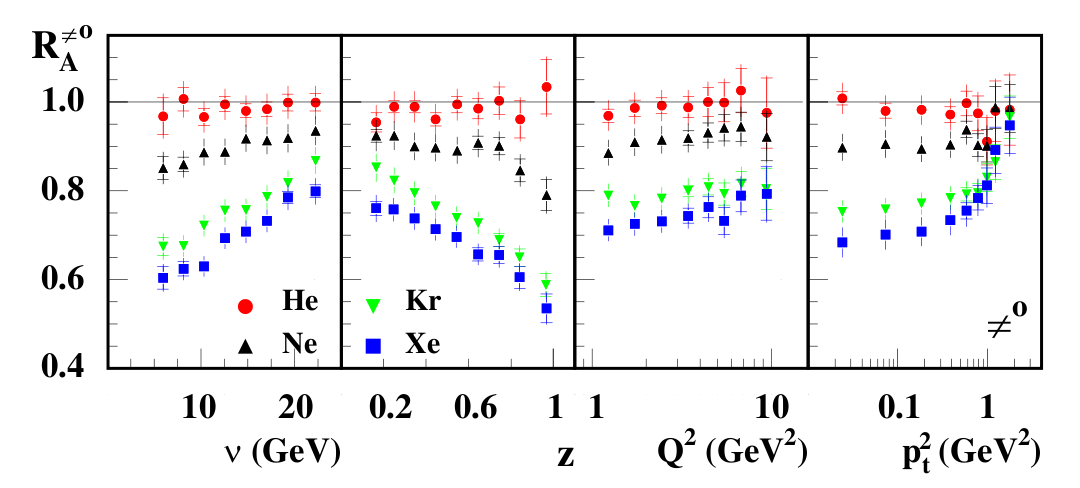
\includegraphics[width=14cm] {fig/Hermes/pi0hermes.png} 
\caption {Multiplicity ratio of $\pi^0$ as a function of various kinetic 
variables from HERMES collaboration \cite{Airapetian:2003mi}}
\label{fig:her1}
\end{figure}

\begin{figure}[htbp]
\centering
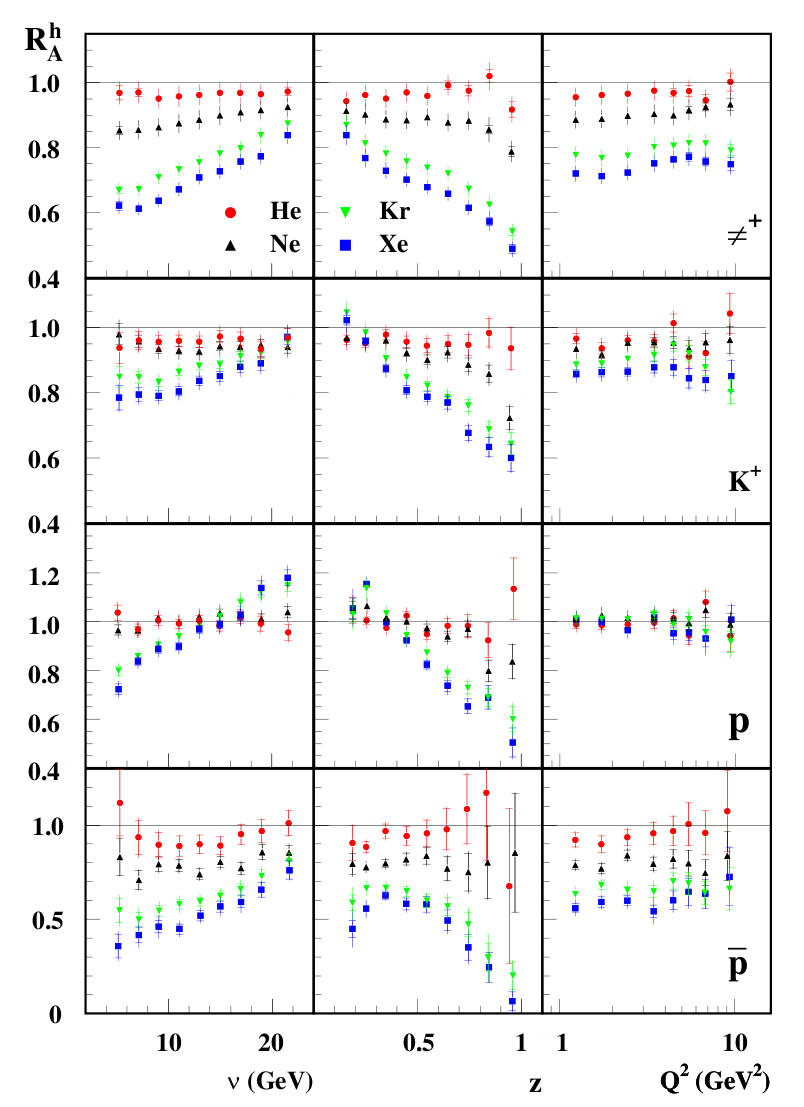
\includegraphics[width=14cm] {fig/Hermes/hermes1.png} 
\caption {Multiplicity ratio of $\pi^+$, K$^+$, protons and anti-protons as a 
function of various kinetic variables from HERMES collaboration \cite{Airapetian:2007vu}}
\label{fig:her2}
\end{figure}

\begin{figure}[htbp]
\centering
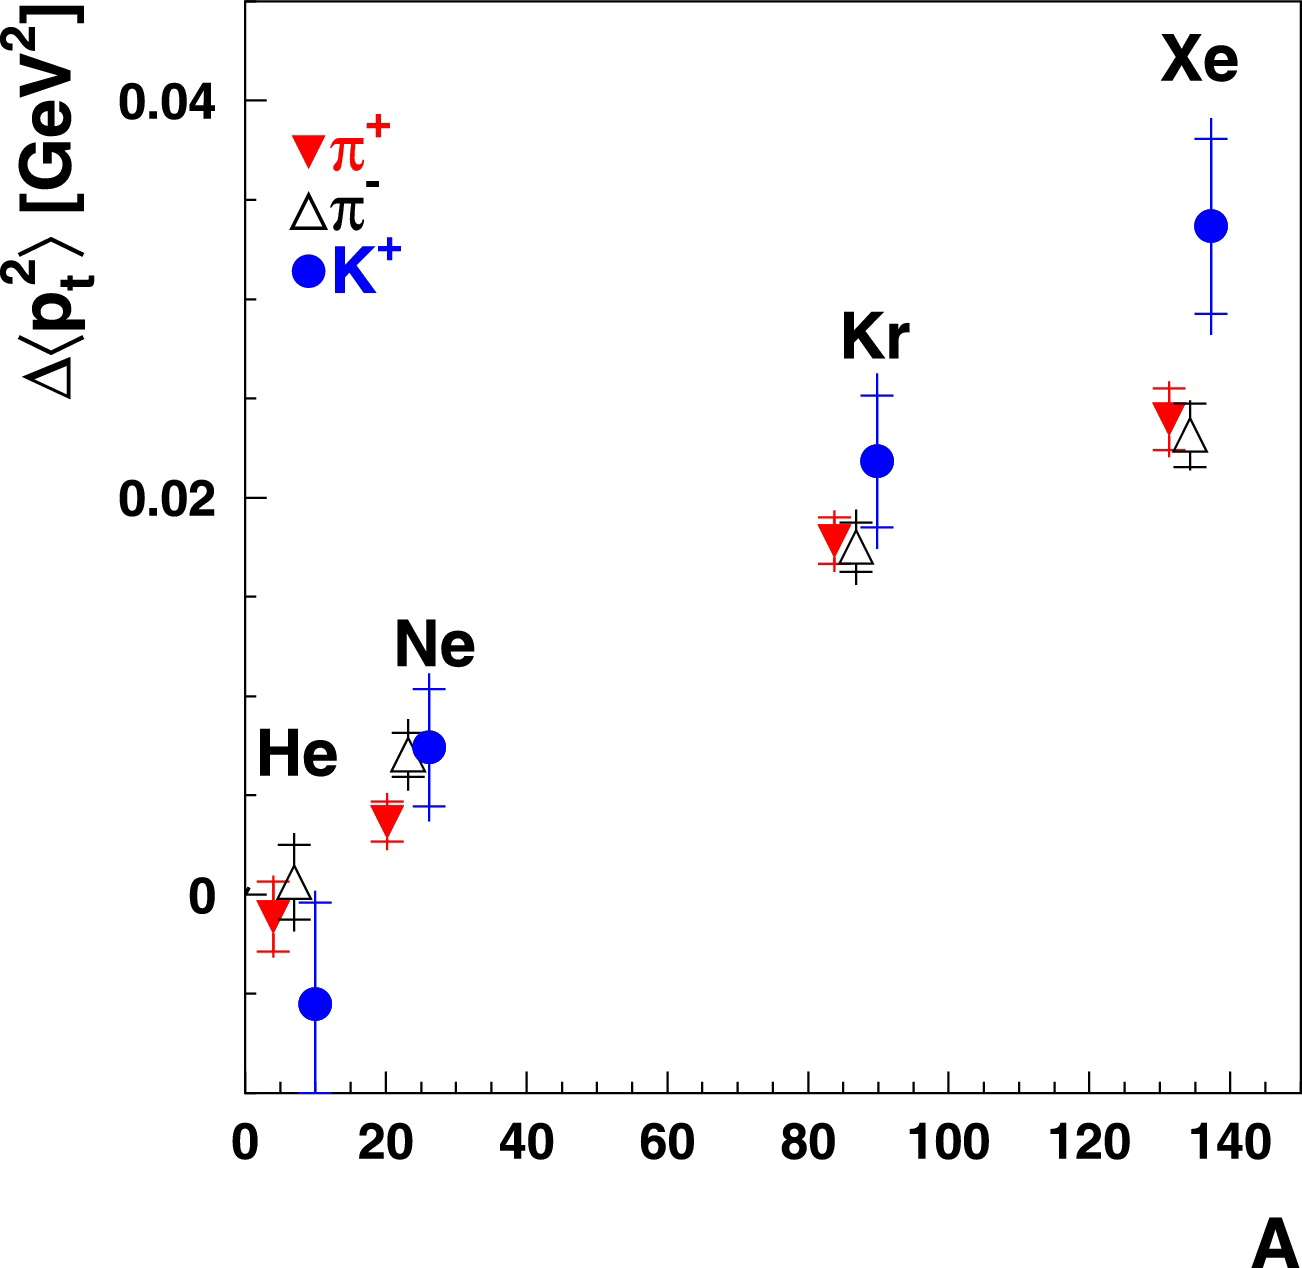
\includegraphics[width=7cm] {fig/Hermes/pthermes.png} 
\caption {Transverse momentum broadening for various particles
from HERMES collaboration \cite{Airapetian:2009jy}}
\label{fig:her3}
\end{figure}

The HERMES data, because of their precision,
permit to have an insight into new features. One can cite the behavior of K$^+$
which have less attenuation than pions (see figure \ref{fig:her1}) but more 
$\Delta \langle P_T^2 \rangle$, it is difficult to reproduce this in 
models where only one stage of hadronization is taken into account to 
explain all effects.
Also the different behaviour of protons compare to anti-protons
(see figure \ref{fig:her1}) is interesting
and need precise analysis even most of the theoritical models do not treat 
baryon hadronization yet.

